\documentclass[a4paper, 10pt]{article}
\usepackage[slovene]{babel}
\usepackage[utf8]{inputenc}
\usepackage{lmodern}
\usepackage[T1]{fontenc}
\usepackage{enumerate}
\usepackage{bbm}
\usepackage{graphicx}
\usepackage{subcaption}
\usepackage{float}

\begin{document}
\begin{titlepage}
\title{Spektralno grupiranje}
\author{Špela Ognjanović in Žiga Trojer}
	\maketitle
\end{titlepage}


\section{Navodilo}
Implement spectral clustering algorithms that use several types of Laplace matrices. Consider unnormalized
spectral clustering, normalized spectral clustering according to Shi and Malik (2000), and normalized spectral clustering according to Ng, Jordan, and Weiss (2002). Generate various data sets or find some examples of real world data and use different types of similarity graphs such as complete graph, the
 $\epsilon$ -neighborhood graph and k-nearest neighbor graph. Compare the results.
Use different methods for determining the optimal number of clusters.

\section{Kratek opis}
Imamo bazo podatkov, naš cilj je te podatke razvrstiti v skupine oz. grupe s podobnimi lastnostmi. Podatke lahko prikažemo z grafi, grafe pa z matrikami. Eden takih primerov je \textbf{matrika sosednosti}, njena razsežnost je n $\times$ n. Element v \textsl{j}-tem stolpcu \textsl{i}-te vrstice pove število povezav, ki povezujejo točki \textsl{i} in \textsl{j}.

Predstavili bomo, kako lahko na različne načine pogrupiramo podatke, podane z množico točk \textsl{\ $x_1$, $x_2$, ... , $x_n$ } z utežmi $w_{i,j} \geq 0$, za $\forall i,j = 1, ... n$ ali razdaljami $d_{i,j} \geq 0$, za $\forall i,j = 1, ... n$. Če o podatkih nimamo veliko informacij, je najlažje, če jih predstavimo z grafom \textsl{G=(V, E)}. Vsako vozlišče $v_i$ predstavlja en podatek \textsl{$x_i$}. Potrebujem matriko, ki določa, kako blizu skupaj sta vozlišči $v_i$ in $v_j$. To matriko imenujemo podobna matrika in jo označimo s \textsl{S}. Dva vozlišča povežemo, če zadoščata danemu pogoju in to ponazorimo v podobnem grafu. Želimo, da imajo vozlišča v istih skupinah čim manjšo utežensot, kar pomeni da imajo podatki podobne lastnosti, sicer velja obratno. Spodaj so opisani trije primeri podobnih grafov, s katerimi bomo operirali.\\
\\
\textbf{Graf $\epsilon$ -ske okolice}\\
Pri $\epsilon$ -ski okolici grafa povežemo paroma vse točke, katerih razdalja je manjša od $\epsilon$. Največkrat je obravnavan kot graf brez uteži, saj nam utež predstavlja predpisana razdalja $\epsilon$.\\
\\
\textbf{Graf k najbližjih sosedov}\\
Cilj je, da povežemo vozlišče $v_i$ z njegovimi k najbližjimi sosedi. Dobimo, da je $v_i$ med k najbližjimi sosedi od $v_j$ ter $v_j$ med k najbližjimi sosedi od $v_i$.\\
\\
\textbf{Poln graf}\\
Je graf, kjer so vsa vozlišča med seboj povezana.\\
\\
Vrnimo se na podobno matriko \textsl{S}. Njene elemente izračunamo s pomočjo neke primerne funkcije. Primer take funkcije je Gaussian Karnelova funkcija, ki nam izračuna oddaljenost dveh vozlišč $v_i$ in $v_j$. Formula za izračun je:$$s(v_i, v_j) = exp(-\textbar\textbar v_i - v_j \textbar\textbar^2 / (2\delta^2)),$$pri čemer parameter $\delta$ opiše razdaljo med vozlišči, podobno kot $\epsilon$ pri grafu epsilonske okolice (vzamemo $\delta$ = 1).  Vrednosti $s_{i,j}$, izračunane po tej meri, so na intervalu [0, 1]. Povejo nam, da manjša kot je vrednost, bolj sta točki oddaljeni. Če je vrednost 0, pomeni, da sta vozlišči daleč narazen. Matrika \textsl{S} je simertrična, saj za toliko kot je vozlišče $v_i$ oddaljena od vozlišča $v_j$, je tudi vozlišče $v_j$ oddaljena od vozlišča $v_i$. Očitno je, da so diagonalni elementi enaki 1.\\
\\
Naslednji korak je izračun \textbf{Laplaceove matrike}. Privzamemo, da imamo utežen, neusmerjen graf $G$. Uteži so prikazane v matriki \textsl{W}, $w_{i,j} \geq 0$, za $\forall i,j = 1, ... n$. Definirajmo še diagonalno degree matriko D: $$ d_i = \sum_{j=1}^n w_{i,j}.$$Glede na normalizirane in nenormalizirane ločimo dva primera Laplaceovih matrik:\\
\begin{enumerate}
\item\underline{Nenormalizirana Laplaceova matrika}, ki se izračuna po formuli $L = D - W$, kjer je \textsl{W} matrika uteži in \textsl{D} diagonalna matrika. Njene lastnosti so:
\begin{enumerate}[i)]
  \item Je simetrična, pozitivno semi-definitna.
  \item Njena najmanjša lastna vrednost je 0, njen pripadajoč lastni vektor je konstanten vektor $\mathbbm{1}$.
  \item Ima n nenegativnih, realni lastnih vrednosti $0 \leq \lambda_1 \leq ... \leq \lambda_n$.
  \item Za vsak $f \in\mathbbm{R}^n$ je $$f'Lf= \frac{1}{2} \sum_{i,j=1}^n w_{i,j}(f_i - f_j)^2.$$
\end{enumerate}

\item\underline{Normalizirana Laplaceova matrika}, sta v bistvu dve matriki, ki sta med seboj povezani, prva je simetrična in se izračuna $L_{sym} = I - D^{-\frac{1}{2}}WD^{-\frac{1}{2}}$, druga pa se izračuna po formuli $L_{rw} = I - D^{-1}W$.
Njune lastnosti so:
\begin{enumerate}[i)]
  \item Sta pozitivno semi-definitni in imata n nenegativnih, realnih lastnih vrednosti.
  \item 0 je lastna vrednost matrike $L_{rw}$, s pripradajočim konstantnim vektorjem $\mathbbm{1}$. 0 je tudi lastna vrednost matrike $L_{sym}$, s pripadajočim lastnim vektorjem $D^\frac{1}{2}\mathbbm{1}$.
  \item $\lambda$ je lastna vrednost matrike $L_{rw}$ z lastnim vektorjem $u$, natanko tedaj, če $u$ reši sistem $Lu = \lambda Du$.
  \item $\lambda$ je lastna vrednost matrike $L_{rw}$ z lastnim vektorjem $u$, natanko tedaj, če je $\lambda$ lastna vrednost matrike $L_{sym}$ z lastnim vektorjem $w = D^\frac{1}{2}u$.
  \item Za vsak  $f \in\mathbbm{R}^n$ je $$f'L_{sym}f= \frac{1}{2} \sum_{i,j=1}^n w_{i,j}(\frac{f_i}{\sqrt{d_i}} - \frac{f_j}{\sqrt{d_j}})^2.$$
\end{enumerate}
\end{enumerate}
S pomočjo Laplaceove matrike ugotovimo, kako dobro smo podatke pogrupirali.

\section{Načrt za reševanje}
Prednost algoritma spectral clustering je, da sestoji na preprosti linearni algebri (npr. izračun lastnih vektorjev, lastnih vrednosti, karakterističnega polinoma, ...). Imamo \textsl{n} točk $x_1$, $x_2$, ... , $x_n$, ki lahko ponazarjajo poljubne objekte. Merimo paroma podobne  \textsl{$s_{i,j}$} =  \textsl{s($x_i$, $x_j$)}, glede na neko simetrično, nenegativno funkcijo (mi uporabimo Gaussian Karnelovo funkcijo). Tako označimo pripadajočo podobno matriko $S=(s_{i,j})_{i,j = 1,..., n}$. Ločimo:
\begin{itemize}
\item[a)] Nenormaliziran algoritem.
\item[b)] Normaliziran algoritem glede na Shi in Malik.
\item[c)] Normaliziran algoritem glede na Ng, Jordan in Weiss.
\end{itemize}
Pri vseh se reševanja lotimo na enak način. Vhodni podatek je podobna matrika $S\in\mathbbm{ R}^{n\times n}$, s  \textsl{k} označimo število grup, ki jih želimo skonstruirati. Nato skonstruiramo enega od podobnih grafov, opisanega v prejšnjem razdelku. Z \textsl{W} označimo uteženo matriko sosednosti. Po formulah izračunamo pripadajočo normalizirano ali nenormalizirano Laplaceovo matriko L. Nato poračunamo prvih k najmanjših pripadajočih lastnih vektorjev matrike L. V matriko U $\in \mathbbm{R}^{n \times k}$ zložimo k lastnih vektorjev v stolpce, po padajočem vrestnem redu glede na pripradajočo lastno vrednost. Vpeljemo zanko for \textsl{i = 1, ..., n}. Nastali vektor $y_i$ predstavlja \textsl{i}-to vrstico matrike U. S pomočjo tega lahko skonstruiramo graf in vidimo, kako dobro smo pogrupirali. Če so točke na grafu zelo narazen pomeni, da smo zelo dobro pogrupirali in obratno.

Množico točk ($y_i)_{i = 1, ..., n}\in \mathbbm{R}^k$ s pomočjo k-means algoritma razvrstimo v grupe $C_1, ..., C_k$. Dobimo $A_1, ..., A_k$, kjer $A_i=\{j\textbar y_i\in C_i\}$. Grupe lahko tudi grafično prikažemo.

Glavna stvar, ki smo jo naredili je, da smo podatke $x_i$ prevedli na $y_i\in \mathbbm{R}^{k}$ in jih tako lažje pogrupirali. S pomočjo lastnih vrednosti Laplaceove matrike lahko izračunamo tudi optimalen k, oziroma optimalno število grup, ki bi jih naj algoritem skonstruiral glede na dano množico podatkov. To naredimo tako, da lastne vrednosti po naraščajočem vrstnem redu upodobimo s točkastim grafom. Optimalno število grup lahko kar odčitamo z grafa, tako, da preštejemo število točk do preskoka. 

\section{Primeri in uporaba}

Uporaba algoritma je zelo razširjena v podatkovni analizi, tudi na vseh naravoslovnih področjih, saj vedno kadar se lotimo nekega problema, kjer so baze podatkov, poskušamo dobiti prvi vtis tako, da pogledamo skupne lastnosti. S pomočjo tega algoritma dobimo podatke zelo dobro posortirane in posledično boljši vtis.\\
\\
Za lažjo predstavo sva se odločila narediti poseben primer, zgled uporabe algoritma na slikah. Sprogramirala sva ga v programu R, tako, da sva najprej vzela sliko z interneta, jo spravila v matriko in nato na njej izvedla algoritem. Rezultati so vidni spodaj na dveh slikah.\\
\\
\begin{figure}[h]
 
\begin{subfigure}{0.5\textwidth}
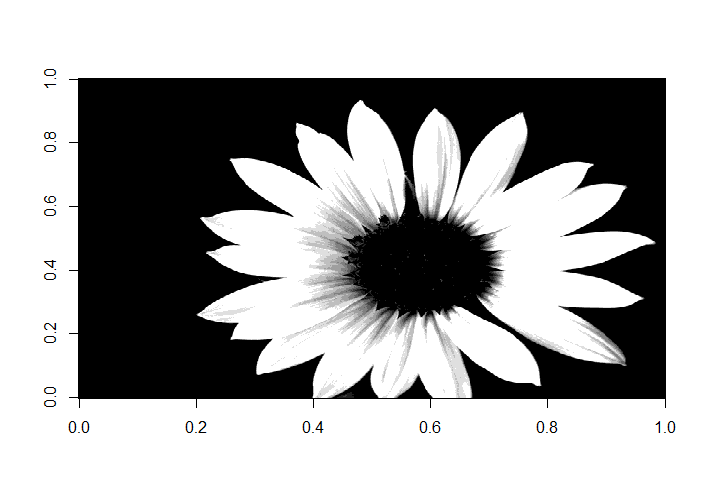
\includegraphics[width=\linewidth, height=4cm]{prva} 
\caption{Prvotna slika}
\label{fig:subim1}
\end{subfigure}
\begin{subfigure}{0.5\textwidth}
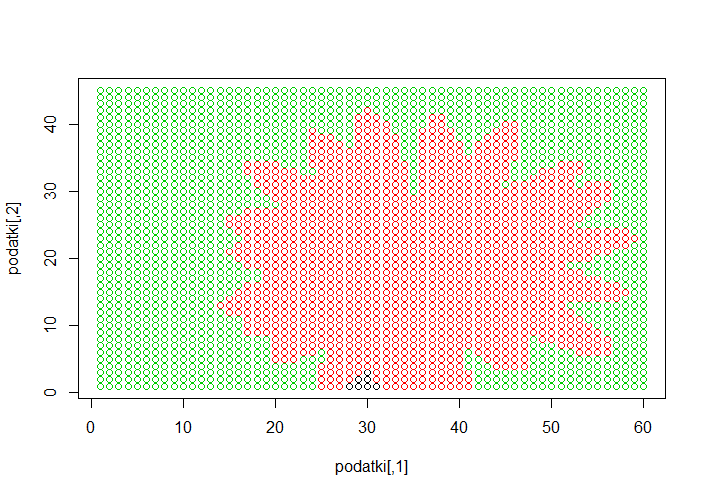
\includegraphics[width=\linewidth, height=4cm]{druga}
\caption{Rezultat}
\label{fig:subim2}
\end{subfigure}
 
\end{figure}


Nadaljuje se




\end{document}

